
\section{Wiederholung Lektüre}

%------------------------------------------------------------------------------
\begin{frame}{Hauptmerkmale eines Modells nach Stachowiak}
% \textbf{Stachowiak,} Herbert: \emph{Allgemeine Modelltheorie}, Wien 1973. 
\subsection{Stachowiak}
\textbf{Stachowiak,} Herbert: \emph{Allgemeine Modelltheorie}, Wien 1973.   
\metroset{block=fill}
\begin{alertblock}{1)~ Abbildungsmerkmal}
\begin{quote} \scriptsize
    „Modelle sind stets Modelle von etwas, nämlich Abbildungen, Repräsentationen natürlicher oder künstlicher Originale, die selbst wieder Modelle sein können.“ 
    %„Originale und Modelle werden hier ausschließlich als Attributklassen gedeutet, die oft die spezielle Gestalt attributiver Systeme erlangen.“ % 131
    „Der Abbildungsbegriff fällt mit dem Begriff der Zuordnung von Modell-Attributen zu Original-Attributen zusammen.“ \parencite[131--132]{stachowiak} % 132
\end{quote}
\end{alertblock}
\begin{alertblock}{2)~ Verkürzungsmerkmal}
\begin{quote} \scriptsize
    „Modelle erfassen im allgemeinen nicht alle Attribute des durch sie repräsentierten Originals, sondern nur solche, die den jeweiligen Modellerschaffern und/oder Modelbenutzern relevant scheinen.“ \parencite[132]{stachowiak}
\end{quote}
\end{alertblock}
\begin{alertblock}{3)~ Pragmatisches Merkmal}
\begin{quote} \scriptsize
    „Eine pragmatisch vollständige Bestimmung des Modellbegriffs hat nicht nur die Frage zu berücksichtigen, \emph{wovon} etwas Modell ist \lbrack{}Abbildungsmerkmal\rbrack{}, sondern auch, \emph{für wen, wann} und \emph{wozu} bezüglich seiner je spezifischen Funktionen es Modell ist.“ \parencite[132]{stachowiak} % 132
\end{quote}
\end{alertblock}

\end{frame}


%------------------------------------------------------------------------------
\subsection{Jannidis, Datenmodellierung}
\begin{frame}{Grundlagen}
\metroset{block=fill}
    \begin{exampleblock}{Formale Modelle}\footnotesize
    \begin{enumerate}
        \item Computer können keine Strukturen in Daten erkennen, sofern diese nicht explizit gemacht werden (z.B. Tabellen) oder programmatisch Regeln definiert werden, wie solche Strukturen aufgezogen werden können (z.B. Sprachverarbeitung).
        \item Zur erfolgreichen Datenverarbeitung ist es daher nötig, Daten in Form formaler Modelle zu strukturieren.
        \item Auszeichnung/Strukturierung erlaubt effizientes Auslesen bestimmter Daten (\emph{Information Retrieval})
    \end{enumerate}
    \end{exampleblock}
\end{frame}

%------------------------------------------------------------------------------
\begin{frame}{Stufen der Datenmodellierung nach Jannidis}
\textbf{Jannidis (Hg.):} \emph{Digital Humanities. Eine Einführung}, Stuttgart 2017: Kap. 7 (\emph{Datenmodellierung}).
\small
\metroset{block=fill}
    \begin{exampleblock}{1) Konzeptuelles Datenmodell}\footnotesize
        \begin{enumerate}
            \item Relevante Entitäten, sowie deren Attribute und Relationen identifizieren	$\to$ relevant in Bezug auf den intendierten Verwendungszweck
            \item Entitäten, Attribute und Relationen in übersichtlicher Form erfassen und visualisieren $\to$ Listen, Tabellen, Diagramme (z.B. Entity-Relationship-Diagramm)
        \end{enumerate}
    \end{exampleblock}
    \begin{exampleblock}{2) Logisches Datenmodell}
        Abbildung des konzeptuellen Modells auf die Struktur einer bestimmten Technologie, z.B. auf ein Datenbank-Schema oder XML-Schema
    \end{exampleblock}
    \begin{exampleblock}{3) Physisches Datenmodell}
        Implementation und physische Repräsentation des Datenmodells auf dem Arbeitsspeicher oder einem externen Speicher in Form bestimmter Datenstrukturen
    \end{exampleblock}
\end{frame}


%------------------------------------------------------------------------------
\begin{frame}{Chen, ER-Modelle}
\textbf{Chen,} Peter: \emph{The Entity-Relationship Model -- Toward a Unified View of Data}, 1976.
\subsection{Chen}
    % ----------------------------------------------
  \begin{columns}[T,onlytextwidth]
  \metroset{block=fill}
\column{0.55\textwidth}\footnotesize
\begin{block}{Entität (Entity)}
    An entity is a „thing“ wich can be distinctly identified. A specific person, company, or event is an example of en entity.
\end{block}

\begin{alertblock}{Beziehung (Relationship)}
    A relationship is an association among entites. For instance, „father-son“ is a relationship between two „person“ enitities.
\end{alertblock}

\begin{exampleblock}{Entitätsmenge (Entity Set)}
    Alle Entitäten derselben Entitätsmenge haben dieselben Eigenschaften (properties).
\end{exampleblock}

    % ----------------------------------------------
    \column{0.35\textwidth}

      \metroset{block=fill}

      \begin{block}{ER-Modell-Bestandteile}
      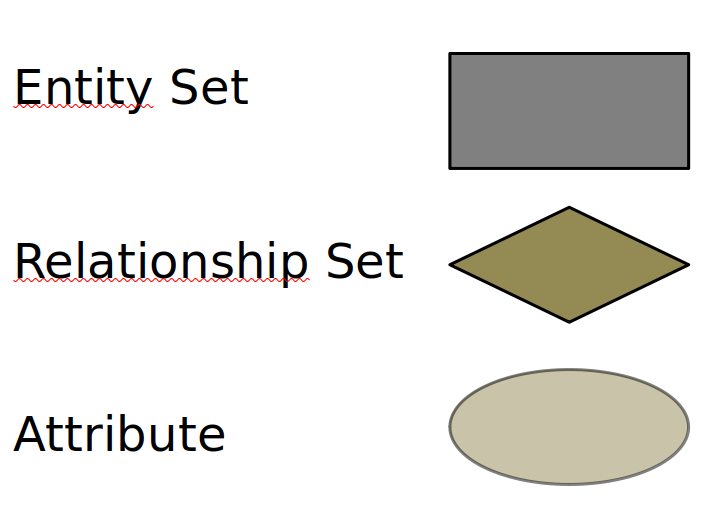
\includegraphics[width=0.9\textwidth]{img/er-modell.png}
      \end{block}
      
      \begin{block}{ER-Modell-Bestandteile}
      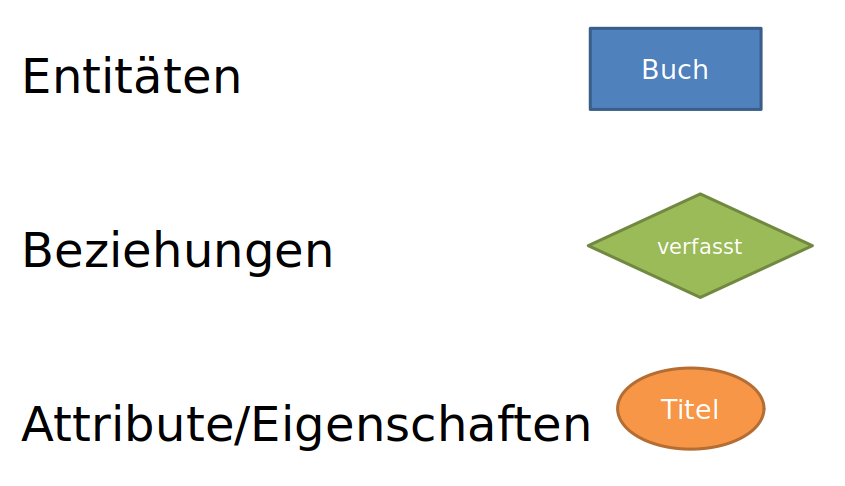
\includegraphics[width=0.9\textwidth]{img/er-bsp2.png}
      \end{block}
  \end{columns}

\end{frame}

%------------------------------------------------------------------------------
\begin{frame}{DH-Einführung, Datenbanken}
\textbf{Jannidis (Hg.):} \emph{Digital Humanities. Eine Einführung}, Stuttgart 2017: Kap. 8 (\emph{Datenbanken}).
\subsection{Jannidis, Datenbanken}
\metroset{block=fill}
%TODO 
\end{frame}


\subsection{Allgemein}
%------------------------------------------------------------------------------
\begin{frame}{Modelle = vereinfachte Repräs. v. Teilen d. realen Welt}
\bg{w3schools}{white}{Model = Abbildung = Repräsenation $\neq$ Original}, sondern nur ausgewählte Teile des Originals werden durch es wiedergegeben bzw. dargestellt. Die Wahl dieser abzubildenden Aspekte der Realität macht die Nützlichkeit oder Repräsentativität für einen bestimmten Anwendungsfall aus.

\bg{w3schools}{white}{Subjektiv \& abstrahiert} $\to$ Muss auf eine spezielle Frage hin erstellt werden und nützt auch nur für diese. Ich kann nie alle Aspekte einer Vase gleichzeitig aufnehmen. Ein Foto zeigt sie nur von einer Seite.

\bg{w3schools}{white}{Disambiguierung und eindeutige Referenzierung} $\to$ ist oftmals für die digitale Repräsentation notwendig, z.B. Normalisierung untersch. Namensformen und Verlinkung des entsprechenden \href{http://d-nb.info/gnd/119287064}{GND-Eintrags}, \href{https://www.geonames.org}{Geonames} -- im Falle von Datenbanken z.B. Primary Keys, Foreign Keys, \dots

\end{frame}
%------------------------------------------------------------------------------



%------------------------------------------------------------------------------
\begin{frame}[allowframebreaks]{Datenmodellierung: Stachowiaks \emph{Allgemeine Modelltheorie}}
\small 

\bg{alert}{white}{Modellbegriff}
„Alle Erkenntnis ist Erkenntnis in Modellen oder durch Modelle und jede
menschliche Weltbegegnung überhaupt bedarf des Mediums Modell“ (Herbert Stachowiak 1973)
\smallskip


\bg{alert}{white}{Datenmodellierung}
Modell =  Ausschnitt aus der realen Welt, allerdings
werden im Modell nur jene Attribute berücksichtigt, die für
meine Fragestellung relevant sind.
 Modell und Realwelt weichen somit voneinander ab.
\smallskip

\bg{alert}{white}{Modell = Abstraktion (=Klasse)}
Konkretisierungen (Kochrezepte, Briefe, Gedichte usw.) eines
Modells werden als Instanzen bezeichnet.
\smallskip

Standardisierte Modelle ermöglichen die gemeinsame
Auswertung, datenübergreifende Suche, Datenaustausch\dots $\to$ nur \bg{alert}{white}{formale Modelle} können digital ausgewertet werden.
\smallskip

\end{frame}


%------------------------------------------------------------------------------
\begin{frame}[allowframebreaks]{McCarty, Modelling}
\metroset{block=fill}
\begin{block}{}
\textbf{McCarty,} Willard: \emph{Modeling: A Study in words and Meanings}, in Schreibman, Siemens and Unsworth (eds.): \emph{A Companion to Digital Humanities},Oxford: Blackwell, 2004, 254--270.
\end{block}
\subsection{McCarty}
\begin{enumerate}
    \item Ein Modell ist eine Repräsentation von etwas, z.B. für Studienzwecke.
    \item Modellierung = heuristischer Prozess in dem Modelle kreiert und verwendet werden, um Probleme zu lösen.
    \item \emph{model of} (beschreibend) vs. \emph{model for} (z.B. Plan zum Hausbau).
    \item Modellierung als experiementeller Vorgang mit dem Ziel der Welterfassung.
    \item Modellierung als iterativer Prozess
\end{enumerate}
\framebreak

\begin{block}{Modellierung}
= heuristischer Prozess; Konstruktion und Manipulation von Modellen
\end{block}

\begin{block}{Modell}
= Repräsentation von etwas (\emph{model of}), oder dient als Entwurf zur Realisierung von etwas Neuem (\emph{model for})
\end{block}
\framebreak

\begin{block}{\cite[255]{mccarty2004}}
\footnotesize
By ``modeling'' I mean the heuristic process of constructing and manipulating models; 
a ``model'' I take to be either a representation of
something for purposes of study, or a design for realizing something new. These two senses follow Clifford Geertz’s analytic distinction
between a denotative ``model of,'' such as a grammar describing the features of a language, and an exemplary ``model for,'' such as an
architectural plan
(Geertz 1973: 93).
\end{block}

\begin{block}{\cite[257]{mccarty2004}}
\footnotesize
In other words, computational models, however finely perfected, are better understood as temporary states in a process of coming to
know rather than fixed structures of knowledge. \punkti computers are essentially modeling machines, not knowledge jukeboxes.
\end{block}
\framebreak

%TODO 

Wichtige Kriterien sind...
...maschinelle Verarbeitbarkeit
...Manipulierbarkeit

Representation
Ein Modell kann entweder die Repräsentation “von” etwas oder die Repräsentation “für”
etwas sein.
Das Modell von etwas, zeigt etwas, das wir noch nicht wissen. Das Modell für etwas gibt
uns etwas, das wir noch nicht haben.
Repräsentationen haben stark mimetische Tendenzen, d. h. sie reproduzieren etwas in
einer greifbaren Form.

Kontext Computing: KR (knowledge representation) bei künstlichen Intelligenzen.
Zur Definition einer Knowledge Representation: First, a knowledge representation is
most fundamentally a surrogate, a substitute for the thing itself, [...] Second, it is a set of
ontological commitments, [...] Fifth, it is a medium of human expression, that is, a language
in which we say things about the world.” In: Randall Davis, Howard Shrobe und Peter Szolovits,
„What Is a Knowledge Representation?”, in: AI Magazine 14/1 (1993), S. 17–33, S. 17. = Davis, Randall,
Howard Shrobe und Peter Szolovits, „What Is a Knowledge Representation?”, in: AI Magazine 14/1
(1993), S. 17–33.

Diagram, Analogy, Map, Simulation, Experiment, Representation

Diagramm repräsentiert Strukturen und Wechselbeziehungen von wichtigen Teilen
eines Objekts.

Eine Simulation imitiert das Verhalten in einer bestimmten Situation / eines
bestimmten Prozess
Werden vor allem zu Lernzwecken eingesetzt
Systeme, welche eine inhärente Komplexität aufweisen (welche kaum vereinfacht
werden kann) werden als Simulationen untersuchbar.

Experiment 
“An action or operation undertaken in order to discover something unknown”
OR “The action of trying anything, or putting it to; a test , trial”
Overlap of “modeling” and “experiment”: in the context of research a model is
an experimental device, modeling an experimental technique
In the mid 19th century: used in the “context of justification” - to the invention
and testing of theories

\end{frame}

